\documentclass[11pt,a4paper]{article}

\usepackage[headsep=1cm,headheight=3cm,left=3.5cm,right=3.5cm,top=2.5cm,bottom=2.5cm,a4paper]{geometry}

\linespread{1.3}
\setlength{\parindent}{0pt}
\setlength{\parskip}{1em}

\usepackage[spanish]{babel}

%% Fuentes personalizadas para utilizar con XeTeX
\usepackage{fontspec}
\setmainfont{IBM Plex Sans}
\setmonofont[Scale=0.9]{IBM Plex Mono}

\usepackage{enumitem}
\setlist[itemize]{leftmargin=*}
\setlist[enumerate]{leftmargin=*}

\usepackage{changepage}

\newcounter{ActCounter}
\newcommand{\act}[1]{\addtocounter{ActCounter}{1}\textbf{\rmfamily ACT-\theActCounter}\quad#1\\}

\usepackage{array}
\usepackage{adjustbox}

\title{Práctica 2: Modelo de casos de uso \large Fundamentos de Ingeniería del Software}
\author{Sofía Almedia Bruno \and José Antonio Álvarez Ocete \and Miguel Lentisco Ballesteros \and Simón López Vico \and José María Martín Luque}

\begin{document}

\maketitle

\section{Introducción}

En el presente documento se muestra el modelo de Casos de Uso obtenido en el proceso de análisis
del sistema para la gestión de un centro médico. El modelo se puede descomponer en dos grandes
paquetes que agrupan las funcionalidades básicas del sistema.

\section{Diagramas de casos de uso} % (fold)

\begin{center}
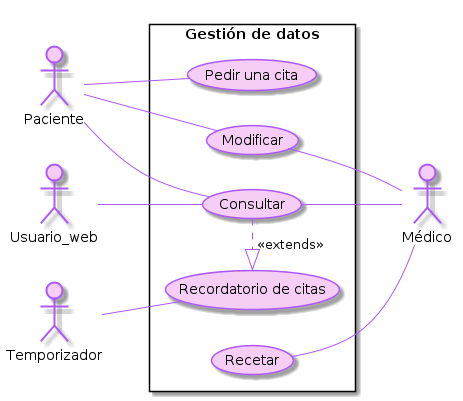
\includegraphics[scale=0.7]{diagramas/gestion_datos}

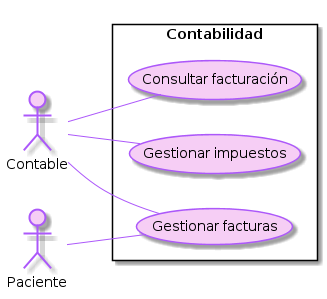
\includegraphics[scale=0.7]{diagramas/contabilidad}
\end{center}

\section{Descripción de los actores}
% PLANTILLA PACIENTE

\begin{table}[h]
\centering
\label{my-label}
\begin{tabular}{l| p{5cm} llll}

\textbf{Actor}           & Paciente & & & & \act \\ 

\textbf{Descripción}     & Paciente adscrito al centro médico que desea pedir cita, consultar su historial o informarse acerca de la clínica & & & & \\
\textbf{Características} & Todos los clientes de la clínica son pacientes  & &  & & \\ 
\textbf{Relaciones}      & & & & & \\ 
\textbf{Referencias}     & & &                                       & \textbf{}                      \\ 
\textbf{Autor}           &  & \textbf{Fecha} &  & \textbf{Versión} & \textbf{}                      \\ 
\end{tabular}
\bigskip
\centering
\label{my-label}
\begin{tabular}{lp{10cm}l}
\textbf{Atributos} &  & \\
\textbf{Nombre}    & \textbf{Descripción} & \textbf{Tipo} \\ \hline
Datos personales   & Identifican al paciente (Id\_paciente, DNI, nombre y apellidos,...)     & \\
Contacto           & Permiten ponerse en contacto con el paciente o algún familiar (teléfono, en caso de emergencia avisar a...) & \\  
Datos médicos      & Información relativa a la salud del paciente (historial médico, grupo sanguíneo, enfermedades previas, alergias,...)            
\end{tabular}
\bigskip
\begin{tabular}{lll}
\textbf{Comentarios} &  &  \\ \hline

\end{tabular}
\end{table}
% FIN PLANTILLA PACIENTE

% PLANTILLA MÉDICO

\begin{table}[h]
\centering
\label{my-label}
\begin{tabular}{l| p{5cm} llll}

\textbf{Actor}           & Médico & & & & \act \\ 

\textbf{Descripción}     & Personal sanitario de la clínica& & & & \\
\textbf{Características} & Puede modificar la información del paciente & & & & \\ 
\textbf{Relaciones}      & & & & & \\ 
\textbf{Referencias}     & & & & & \\ 
\textbf{Autor}           &  & \textbf{Fecha} & & \textbf{Versión} & \\ 
\end{tabular}
\bigskip
\centering
\label{my-label}
\begin{tabular}{lll}
\textbf{Atributos} &  & \\
\textbf{Nombre}    & \textbf{Descripción} & \textbf{Tipo} \\ \hline
Datos personales   &  Identifican al médico (Id\_médico, DNI, nombre y apellidos,...)     & \\
Datos laborales    & Relativos a su trabajo (horario, sueldo, vacaciones,...)&              
\end{tabular}
\bigskip
\centering
\begin{tabular}{lll}
\textbf{Comentarios} &  &  \\ \hline
\end{tabular}
\end{table}

% FIN PLANTILLA MÉDICO
\section{Descripción de los casos de uso}

% Usar la plantilla general

\section{Diagrama de paquetes}

	
\end{document}
